\section{Cross-Level Synthesis}
\label{sec:synthesis}

The five capability levels separate task form, but the field's larger patterns emerge only when those levels are crossed with clinical application, architecture, and evidence. These secondary lenses do not reclassify papers. They show where particular capabilities concentrate, which model designs recur across levels, and where SATO-V evidence most often breaks. Figure~\ref{fig:landscape} summarizes the capability--application landscape, while Table~\ref{tab:cross-level-synthesis} condenses the principal cross-level conclusion.

\begin{figure}[t]
\centering
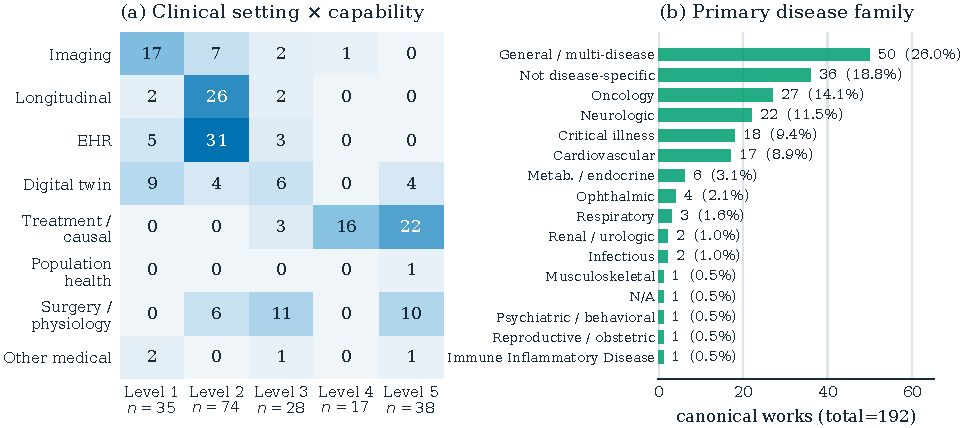
\includegraphics[width=\linewidth]{figures/fig_landscape.pdf}
\caption{Capability and clinical context. \textbf{(a)} Primary clinical application crossed with the non-cumulative Level~1--5 categories for implemented clinical canonical works with sufficient evidence for adjudication ($n{=}\MedicalImplementedTotal$). \textbf{(b)} Primary disease-family distribution for the same works. Contextual, duplicate-version, unresolved, and non-transition records are excluded.}
\label{fig:landscape}
\end{figure}


\subsection{Capability $\times$ Clinical Application}

Imaging supplies a large share of the state-representation and future-prediction literature. Its dense observations and mature generative models make Level~1 and Level~2 systems comparatively accessible. Imaging also reaches Level~3 through treatment-conditioned disease generation and acquisition control, and Level~5 through guidance or planning. The limiting evidence changes across this progression. At lower levels, patient identity and biological fidelity are central; at action-aware levels, the main question is whether conditioning represents an executable intervention; in planning, image quality must be connected to a decision-relevant endpoint.

EHR and patient-trajectory modeling spans future prediction, action-conditioned simulation, counterfactual estimation, and planning. The recurring difficulty is that state, action, and outcome can all appear as tokens in the same sequence. This makes implementation flexible but interpretation fragile. A model can forecast a medication, condition on a medication, estimate its potential outcome, or use simulated outcomes to select it. These are four different contracts. EHR models therefore benefit most from explicitly separating patient state, observation process, clinician behavior, and the intervention interface.

Longitudinal disease models bridge imaging and treatment simulation. Natural-history forecasting is Level~2; treatment-aware rollout can reach Level~3; causal comparison requires Level~4 evidence; and optimization produces a Level~5 system. Oncology and neurology are prominent because repeated imaging and clinically meaningful progression are available, but missing visits, treatment switching, censoring, and long horizons complicate validation. A visually plausible progression is not equivalent to patient-specific response.

Surgical, robotic, acquisition, and physiological systems have comparatively clear actions. Tool motion, probe movement, acquisition rotation, and controlled physiological inputs can be instrumented and repeated. This often makes the Level~2/Level~3 boundary easier to judge than in EHR. The weak point moves to physical consistency, safety, and outcome relevance. A high-fidelity training simulator may be valuable while remaining inappropriate for real-time clinical control. These applications demonstrate that clear action semantics are necessary but not sufficient for clinical-action validity.

Digital twins cut across all five levels. They can initialize a patient state, forecast natural history, simulate interventions, support counterfactual reasoning, or guide optimization. Treating the term as an independent capability would therefore hide more than it reveals. The useful questions are what is twinned, how the state is updated, which actions are exposed, what model drives the transition, and how the resulting decision is validated. A focused mechanistic twin with tested intervention response can be more informative than a broad multimodal architecture with only static prediction.

\subsection{Capability $\times$ Model Architecture}

No architecture maps to one level. Diffusion and flow models can reconstruct current observations, predict future images, or generate treatment-conditioned futures. Autoregressive transformers can forecast EHR events, emulate action-conditioned patient trajectories, or provide an environment for planning. Latent state-space models can support natural history, intervention response, and model-predictive control. Mechanistic models can serve prediction, causal simulation, or optimization depending on how actions and decisions enter. Graphical or symbolic structure reaches the counterfactual category only when it participates in a defensible identification or structural contract.

Architecture nevertheless shapes characteristic failure modes. Autoregressive systems risk reproducing documentation and clinician behavior instead of patient dynamics. Diffusion and video models risk substituting perceptual realism for biological or physical validity. Latent state-space models must address observability and uncertainty. Mechanistic systems must justify parameters, structural assumptions, and patient-specific updating. Hybrid foundation systems must state which component carries state, dynamics, intervention response, and validation. These patterns motivate a qualitative architecture lens, but not architecture prevalence claims before the codebook has been normalized.

The most promising designs are likely to combine strengths rather than select a single family. Learned representations can absorb multimodal observations; state-space structure can separate dynamics from measurement; mechanistic constraints can encode known physiology or geometry; causal components can define treatment comparisons; and planners can use uncertainty to limit action search. Hybridization is useful only when component responsibilities remain inspectable. A large multimodal system that obscures the action pathway is harder to validate than a narrower model with a clear contract.

\subsection{Capability $\times$ SATO-V Evidence Quality}

State is generally the strongest SATO-V component. Imaging, EHR, waveform, and surgical-scene representations are often well specified. Action and validation are weaker. At Level~2, the central issue is whether forecast accuracy reflects the patient or the record-generating process. At Level~3, the action may be explicit while its empirical support and causal meaning remain uncertain. At Level~4, the missing potential outcome forces reliance on assumptions, trials, quasi-experiments, mechanistic constraints, or semi-synthetic anchors. At Level~5, model and reward error are amplified by optimization, while evaluation is often retrospective or simulator-based.

Outcome validity cuts across the ladder. A future image, event token, physiological state, or simulated reward may be an appropriate technical target. The claim becomes miscalibrated when that target is treated as a patient-centered outcome without a validated link. Validation should therefore be decision-aligned rather than uniformly ``stronger'' at higher levels. A Level~1 state model may require external representation transfer; a Level~2 forecaster requires horizon-specific calibration; a Level~3 simulator requires action-sensitivity and support tests; a Level~4 estimator requires identification and sensitivity evidence; and a Level~5 planner requires policy-level and prospective evaluation.

\subsection{What the Field Has Actually Achieved}

The field has clearly moved beyond static prediction. Future-state modeling is established across imaging, EHR, and physiology, and action-conditioned simulation is visible in treatment, acquisition, and embodied settings. Model-based planning is also implemented in several clinical and simulator-mediated systems. The evidence is less complete than the capability labels suggest. Counterfactual identification remains concentrated in adjacent causal methods, and prospective decision-level validation remains uncommon relative to the clinical ambition of the work.

The principal gap is therefore not a missing generative backbone. It is the integration of four elements that are currently distributed across different literatures: rich patient state, executable action, credible alternative-outcome reasoning, and decision-aligned validation. Imaging and foundation models contribute representation and generation; causal methods contribute estimands and assumptions; mechanistic twins contribute structural constraints; model-based control contributes operational decision loops. A clinically credible medical world model will need these elements to meet in one inspectable evidence chain.

\begin{table*}[t]
\caption{Cross-level evidence synthesis. Capability identifies the implemented task form; the remaining columns summarize what the reviewed literature supports and what must change before a stronger clinical interpretation is justified.}
\label{tab:cross-level-synthesis}
\centering
\small
\setlength{\tabcolsep}{4pt}
\renewcommand{\arraystretch}{1.08}
\begin{tabularx}{\textwidth}{@{}p{2.6cm}p{4.0cm}p{4.0cm}X@{}}
\toprule
\textbf{Level} & \textbf{Observed achievement} & \textbf{Main evidence gap} & \textbf{Next threshold} \\
\midrule
Level 1: state representation & Clinically useful image, EHR, physiological, and mechanistic state construction. & No directed transition; representation may encode nuisance or observation-process structure. & A calibrated future target supported by a stable, uncertainty-aware state. \\
Level 2: future prediction & Longitudinal images, patient events, disease states, and physiological trajectories can be forecast. & Record prediction is often conflated with patient dynamics; long-horizon and external calibration are limited. & An executable action that enters the transition and changes an evaluated future. \\
Level 3: action-conditioned simulation & Treatment, acquisition, surgical, and physiological actions can control simulated futures. & Conditioning may reproduce selection bias or superficial action correlations rather than intervention response. & An explicit alternative-outcome estimand with identification or structural support. \\
Level 4: counterfactual reasoning & Causal sequence, survival, and mechanistic methods estimate outcomes under alternative interventions. & Both potential outcomes are unobserved; support, confounding, and individual-level uncertainty remain difficult. & Operational use of a validated model in action ranking or selection, with decision-error analysis. \\
Level 5: planning and control & World models support treatment planning, policy evaluation, acquisition guidance, and simulator-mediated control. & Optimization amplifies transition bias, unsupported actions, and reward misspecification; prospective evidence is sparse. & Support-aware planning, calibrated abstention, external validation, and patient-relevant prospective evaluation. \\
\bottomrule
\end{tabularx}
\end{table*}

